\documentclass[../main.tex]{subfiles}
\begin{document}

\ifSubfilesClassLoaded{
	\mainmatter
	\setcounter{chapter}{1}
}{}

\chapter{SeaQuest Experiment}
\label{ch:seaquest}

\section{Introduction}
SeaQuest is a fixed-target experiment utilizing the \SI{120}{\GeV} proton beam
from the Fermilab Main Injector. Details of the SeaQuest spectrometer can be
found in Ref.\ \cite{aidala2019}. A schematics of the spectrometer is shown in
Fig.\ \ref{fig:spectrometer}. The target system consists of seven
interchangeable targets, including a flask with liquid hydrogen, a flask with
liquid deuterium,an empty flask (vacuum), solid carbon, iron, and tungsten
targets as well as a space with no target (air). The targets are interchanged
periodically to reduce systematic uncertainties in the measured cross section
ratios for different targets.

The spectrometer consists of two magnets and four tracking stations. FMag,
placed \SI{104}{\cm} downstream the target, is a \SI{5}{\m} solid iron magnet
that acts as the beam dump as well as a focusing magnet. It is then followed by
the first tracking stations. Stations 1, 2 and 3 each consists of plastic
scintillator hodoscopes and drift chambers. An open air dipole magnet (KMag) is
placed between station 1 and station 2. The vertical magnetic field from both
magnets bends the muons horizontally, allowing the measurement of the momentum
of the muons. Downstream of station 3, there is a 1 m iron wall acting as a
hadron absorber. Station 4 is located behind the hadron absorber and acts as a
muon identifier. Station 4 consists of a hodoscope array and 4 layers of
proportional tube planes. Tracks that pass through the hadron absorber and
produce hits on station 4 are assumed to be from muons.
\pdfmargincomment{Should there be a dedicated section on the spectrometer?
	how much detail of the spectrometer is need?
}

\begin{figure}[htbp!]
	\centering
	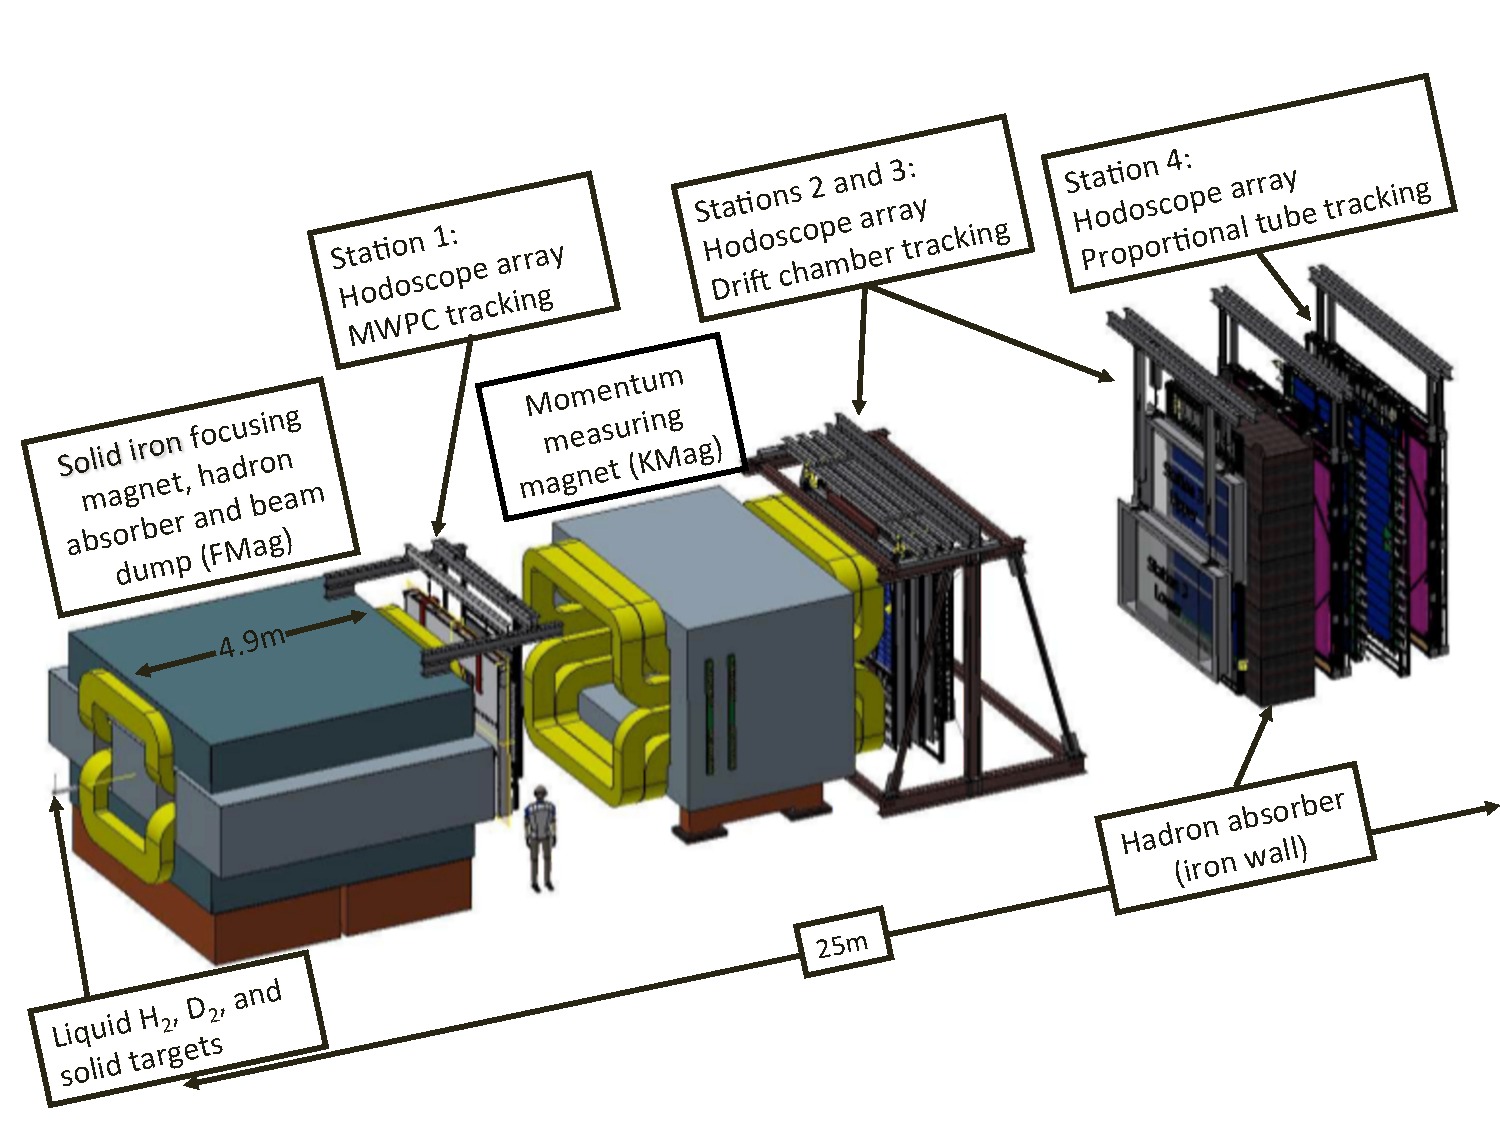
\includegraphics[width=0.6\linewidth]{SeaQuestSpectrometer}
	\caption{schematics of the SeaQuest spectrometer. Taken from Ref.\
		\cite{aidala2019}}
	\label{fig:spectrometer}
\end{figure}


\section{Beam}
\pdfmargincomment{A brief description of the beam structure, how the beam intensity
	is monitor. And finally says that the varying instantaneous beam intensity
	allows us to do intensity extrapolation which will be discussed in next
	chapter}
The layout of the Fermilab accelerator complex is shown in Fig.\ \ref{fig:complex}.
SeaQuest received its \SI{120}{\GeV} proton beam from the Fermilab Main Injector.
The proton beam originate from a direct-extraction magnetron hydrogen ion source,
which produce a \SI{35}{\keV} negative hydrogen ion beam. It is then accelerated
to \SI{750}{\keV} using Radio-frequency Quadrupole. Then the Linac accelerate the
$H^-$ ions to \SI{400}{\MeV}. The $H^-$ ions are then sent through a stripping foil
to remove the electrons. The resulting proton beam then circulates in the Booster
accelerator and accelerates to \SI{8}{\GeV}. The \SI{8}{\GeV} proton beam is
further accelerated by the Main Injector to \SI{120}{\GeV}. The proton beam is
extracted from the Main Injector using a process known as resonant extraction to
provide a lower intensity beam over a 5 second spill. The extracted beam, which
is sent to SeaQuest, retains the \SI{53.1}{\MHz} structure of the Main
Injector RF frequency, dividing the beam in to ``RF buckets'' that are less than
\SI{2}{\ns} long and occur every \SI{18.8}{\ns}.
\begin{figure}[htbp!]
	\centering
	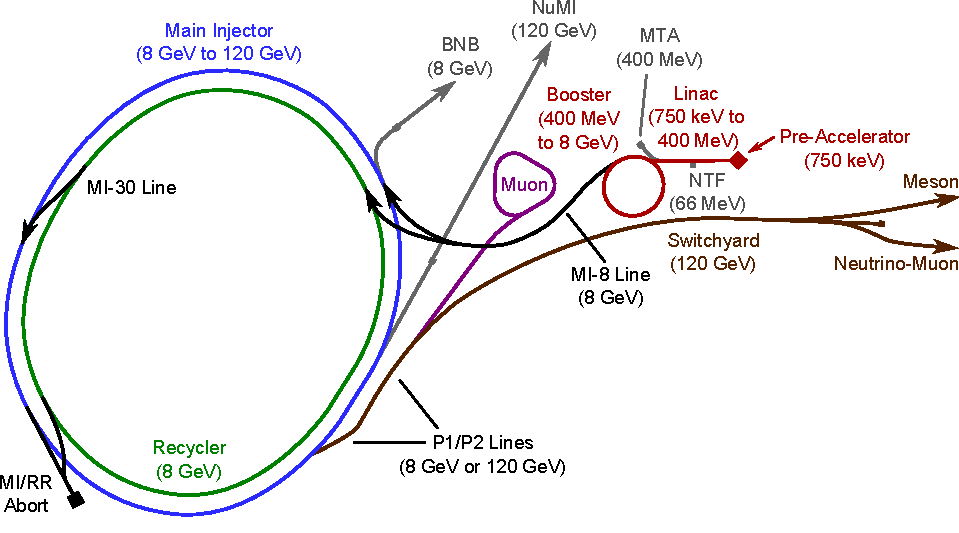
\includegraphics[width=0.6\linewidth]{Fermilab-complex}
	\caption{Layout of the Fermilab accelerator complex. Taken from Ref.\ \cite{concept-book}}
	\label{fig:complex}
\end{figure}
However the number of protons in each bucket varies greatly during the spill, as
is shown in Fig.\ \ref{fig:intensity}.
\begin{figure}[htpb!]
	\centering
	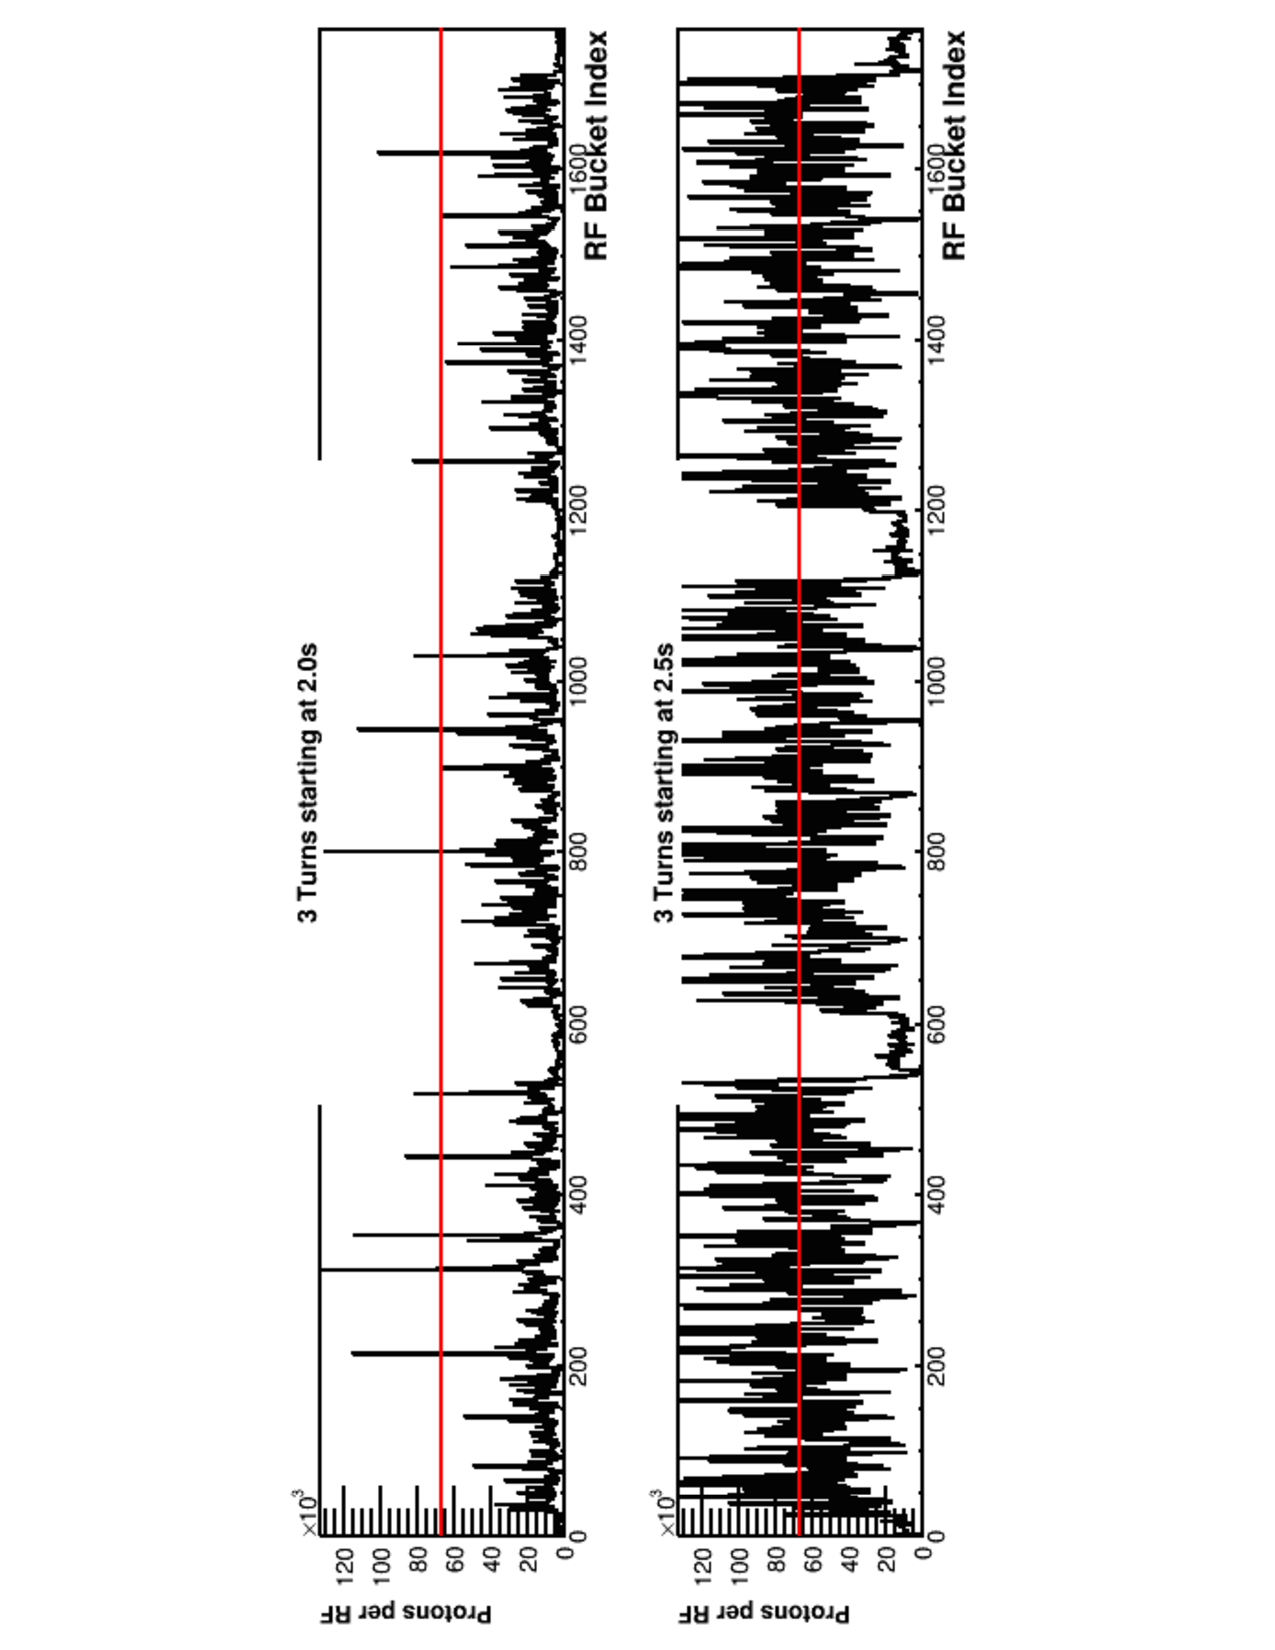
\includegraphics[width =0.8\linewidth, angle =270]{beam_intensity}
	\caption{The beam intensity measured by the Beam DAQ Cerenkov counter every
		bucket. Taken from Ref.\ \cite{aidala2019}}
	\label{fig:intensity}
\end{figure}

\subsection{Beam Intensity Monitor}
The beam intensity is monitored using a Cerenkov counter, shown in Fig.\ \ref{fig:BIM}.
\begin{figure}[htbp!]
	\centering
	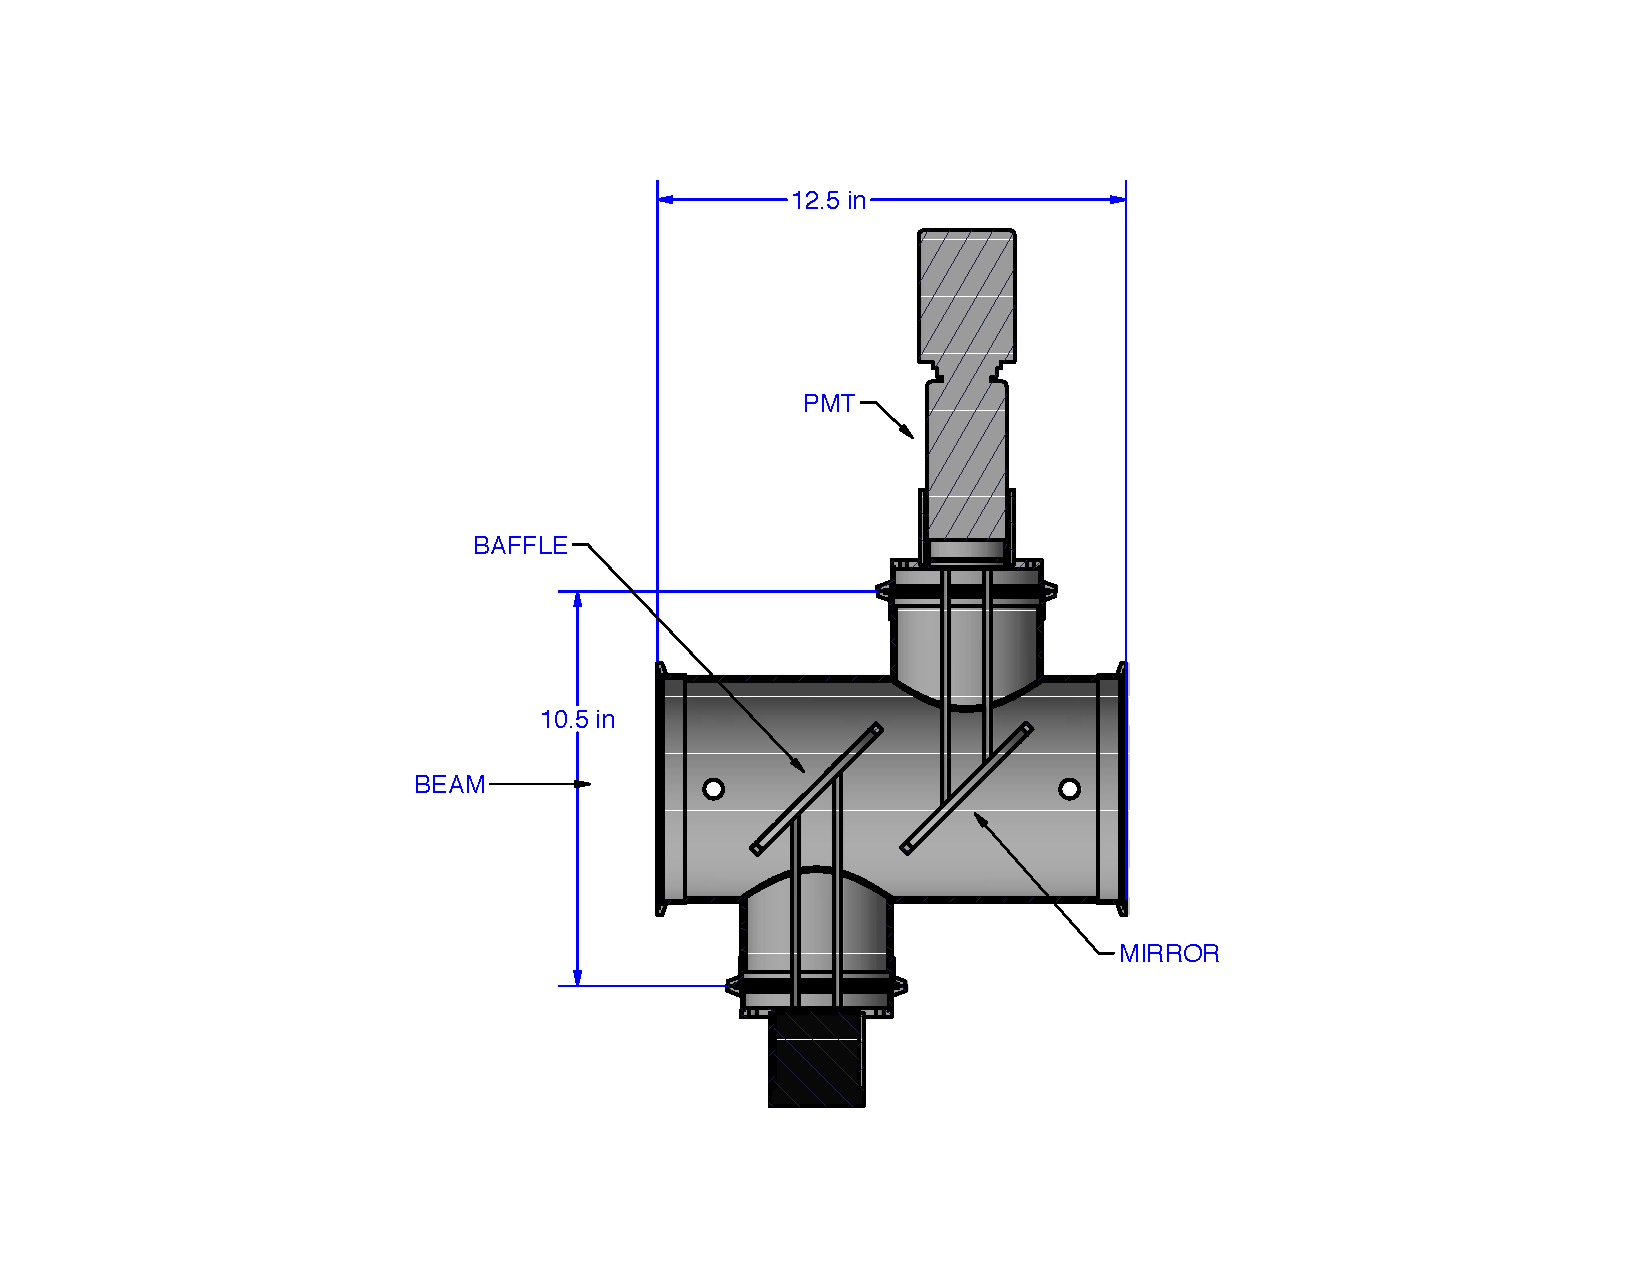
\includegraphics[width=0.6\linewidth]{BIMCerenkov}
	\caption{The Beam Intensity Monitor (BIM) Cerenkov counter. Taken from Ref.\
		\cite{aidala2019}.}
	\label{fig:BIM}
\end{figure}
A aluminized Kapton mirror reflect the Cerenkov light, produced when the proton beam
passing through the radiator, into a single photomultiplier tube. The signal is then
sent to a custom ``QIE'' (Charge Integrator and Encoder) module. This custom module
is clocked with the Main Injector RF, and is capable to recording the beam intensity
of each RF bucket for the entire spill. The QIE module is linked to the trigger
system, and would raise a trigger inhibit when the beam intensity is above a
threshold. The module is also read out by the Beam DAQ, which provides the (a)
integrated beam intensity for entire spill; (b) integrated beam while inhibit is
asserted at trigger logic; (c) integrated intensity during dead time; (d) a snapshot
of the beam intensity close in time to the trigger; and (e) a complete record of the
bucket-bucket intensity for the entire spill.

The ability to record the numbers of proton in each bucket allows us the obtain the
yield ratios as a function of the instantaneous intensity, which will be discussed
further in Sec.\ \ref{M-sec:extrapolation}


\section{Target}
\pdfmargincomment{list the properties of the targets. Some past thesis quoted the
	wrong number. Check PDG}
The SeaQuest target is place between the Beam Intensity Monitor and the front face
of FMag. The target system consists of two liquid targets, hydrogen and deuterium,
and three solid targets, iron, carbon and tungsten. Each solid target is divided
into \num{3} discs of equal length, and are spatially separated along the beam
direction to minimize variation in acceptance between liquid and solid targets.
To account for background originating from the interaction with the instruments,
there are also two calibration targets, an empty vacuum filled flask, known as
empty flask, and the solid target holder, known as no-target. The different targets
are mounted on a motorized table, which allows the targets to be interchanged
between spills to minimized systematic effect due to spectrometer performance.
The properties of the targets and the spills per cycle of each target positions
are listed in Table.\ \ref{table:target}.
\pdfmargincomment{schematics of target system}


\begin{table}[h!]
\caption{SeaQuest target configuration}
\label{table:target}
\begin{tabular}{|c|c|c|c|c|c|}
\hline
Target      & Position & Density (\unit{\g\per\cm\cubed}) & length (\unit{\cm}) & interaction length   (\unit{\g\per\cm\squared}) & spill/cycle \\ \hline
\ce{LH_2}   & 1        & \num{0.071}                      & \num{50.8}          & \num{52.0}                                      & 10          \\ \hline
Empty Flask & 2        & -                                & -                   & -                                               & 2           \\ \hline
\ce{LD_2}   & 3        & \num{0.1634}                     & \num{50.8}          & \num{71.8}                                      & 5           \\ \hline
No target   & 4        & -                                & -                   & -                                               & 2           \\ \hline
Iron        & 5        & \num{7.87}                       & \num{1.905}         & \num{132.1}                                     & 1           \\ \hline
Carbon      & 6        & \num{1.80}                       & \num{3.322}         & \num{85.8}                                      & 2           \\ \hline
Tungsten    & 7        & \num{19.30}                      & \num{0.953}         & \num{191.9}                                     & 1           \\ \hline
\end{tabular}
\end{table}

\section{Tracking Station}
The SeaQuest detector system is separated into four tracking stations. Stations \num{1},
\num{2} and \num{3} comprise of hodoscopes and drift chambers. Whereas station \num{4}
comprises of hodoscope and proportional tubes. The hodoscopes in each stations provides
a fast signal for triggering whereas the drift chambers provide good spatial resolution 
for pprecise reconstruction. The proportional tubes at station 4 is also used for muon
identification.

\subsection{Hodoscope}
\pdfmargincomment{why are there 2 y hodo in St4? Lower rate at St4? }

\subsection{Trigger System}
\pdfmargincomment{how is the charge determined?}

\subsection{Drift Chambers}

\subsection{Proportional tubes}
\pdfmargincomment{https://doi.org/10.1080/08929880802335758}

\ifSubfilesClassLoaded{ \printbibliography[heading=bibintoc,title={References}]}{}
\end{document}
